\subsection{Funktionsprinzip}

Eine Spule, oder der Anschaulichkeit halber, eine Leiterschleife, befindet sich in einem magnetischen Feld (Siehe Abbildung).\footnote{Abbildung von LeiFi Physik: \url{http://www.leifiphysik.de/sites/default/files/medien/generator02_elmagnetindukt_ver.gif}}

\begin{figure}[h!]
	\centering
	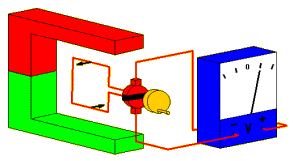
\includegraphics[width=0.6\textwidth]{GeneratorSchema}
	\caption{Schema eines Wechselstromgenerators mit Kommutator} 
\end{figure}


Die Leiterschleife wird angedreht und der sich in der Grafik oben befindende Teil der Schleife bewegt sich senkrecht zu den Feldlinien des Magnetfeldes. Somit wirkt auf die Teilchen die Lorentzkraft, gemäß Linker-Hand-Regel (Siehe \referenz{sec:lorentzkraft}). Im Beispiel ist der Plus-Pol am oberen Ende und der Minus-Pol am unteren Ende.

Wenn sich die Schleife nun um 90\degree{} gedreht hat, bewegen sich beide Pole kurzzeitig parallel zu den Feldlinien; die Elektronen in der Schleife werden nicht mehr beeinflusst und es liegt keine Spannung mehr an. Der sinusförmige Spannungsgraph resultiert aus der Bewegung dazwischen.

Nach weiteren 90\degree{} ist das ursprünglich obige Stück Schleife unten und nun der Minus-Pol. Das ist der Grund für die negativen Passagen der Spannungskurve.


\subsubsection{Kommutator}

Ein Kommutator, wie in der Abbildung, kehrt die Polarität der Leiterschleifenteile bei jeder halben Umdrehung um, sodass es nie eine negative Spannung gibt. Der schwarze Teil ist ein Isolator und die Backen, die oben und unten liegen, schleifen über Bürsten am sich drehenden Kommutator.

Die Spannungskurve\footnote{„Betrag von sinx“ von Till Blaha - Eigenes Werk. Lizenziert unter Gemeinfrei} ist dann der Betrag: $|\sin x|$:

\begin{figure}[h!]
	\centering
	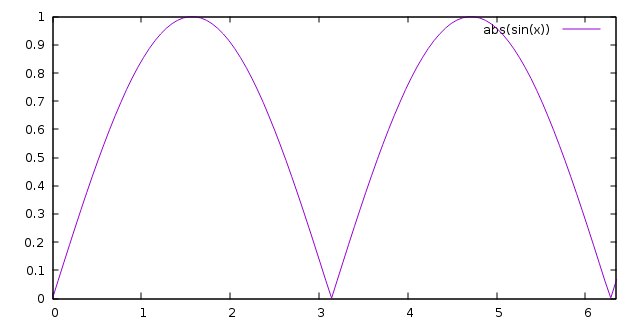
\includegraphics[width=0.7\textwidth]{Betragsinx}
	\caption{Ideale Spannungskurve mit einem Kommutator.} 
\end{figure}


\subsection{Induktionsspannung bestimmen}

Um die maximale Spannung (Amplitude), zu bestimmen, muss die Feldstärke des Magnetfeldes, die Windungszahl, Fläche und Induktivität der Spule sowie die Drehfrequenz bekannt sein. Die Gleichung ist analog zur generellen Induktionsspannung (Siehe \gleichungsreferenz{eq:InduGe}) $U_{ind} = -N \frac{d(B \cdot A)}{dt}$:

\begin{equation}	\label{eq:hatU}
	\hat{U} = NBA \cdot \omega
\end{equation}

\noindent Daraus folgt für einen beliebigen Zeitpunkt:

\begin{align}		\label{eq:hatUbeliebig}
\begin{split}
	U(t) &= \hat{U} \cdot sin(\omega \cdot t) \\
	U(t) &= NBA \cdot \omega \cdot sin(\omega \cdot t)
\end{split}
\end{align}



